%% Updated by using Latex

\documentclass[english]{article}
\usepackage[T1]{fontenc}
\usepackage[latin9]{inputenc}
\usepackage{graphicx}
\usepackage{babel}
\begin{document}
\title{CrowdEgress: A Multi-Agent Simulation Platform for Pedestrian Crowd}

\maketitle
\author{Peng Wang, Xiaoda Wang, Peter Luh, Neal Oldman}

\begin{abstract}
This manual introduces a simulation tool to study crowd evacuation
behavior. The simulation platform is compatible to the well-known
tool FDS+Evac (Version 5 and 6), and the input data in FDS+Evac could be imported into our simulation framework to create compartment geometry. Most importantly, we intent to integrate real-world human data into our simulation to investigate human behavior in emergency evacuation, such as pre-evacuation behavior, exit-selection activities, grouping effect and so forth.  
\end{abstract}

\section{Introduction}

The program mainly consists of four component: User Interface, Simulation
Core, Data Tool, Visualization Tool.  

\textbf{User Interface}: The user interface is written in tkinter
in ui.py. Please run ui.py to enable a graphic user interface (GUI)
where one selects the input files, initialize compartment geometry,
and configure or start a simulation. An alternative method is using
main.py to directly start a simulation without GUI. Currently
there is a simple version of GUI and it needs to be improved in several
aspects.

\textbf{Simulation Core}: The multi-agent simulation is implemented
in simulation.py. The component is packed in a class called simulation
class, and it computes interaction of four types of entities: agents,
walls, doors and exits. The agent model is described in agent.py,
while walls, doors and exits are coded in obst.py. The agent-based
model is an extension of the well-known social force model\cite{Helbing00,Helbing02,Helbing95}.
The model aims at investigating protypes of pedestrian behavior in
crowd evacuation. The core algorithm is still being studied and improved.
This is an interesting study topic, which refers to Newton particles,
complex systems and behavioral science. Your contributions are much
welcome.

\textbf{Data Tool}: This component reads in data from input files,
and write data to output files. The input data is written by users
in either csv files or fds input files. Agents must be specified in
.csv file while walls, doors or exits can be described either in csv
file or read from standard fds input file. The simulation output is
written into a binary file, which is compatible to the fds output
data (fds prt5 data format). 

\textbf{Visualization Tool}: The visulization component is packed
in draw\_func.py and currently pygame (SDL for python) is used to
develop this component. Users can select to visualize the simulation
as it runs, or visualize the output data after the simulation is complete.
If anyone is interested, please feel free to extend the module or
try other graphic libraries to wrtie a visulization component.

\section{About Simulation Model}

Agent-based model (ABM) describes interactions among individual agents
and their surroundings. In the simulation core there are four types
of entities: agents, walls, doors and exits, and their interactions
are illustrated in Figure 1.

\begin{figure}
\centerline{\includegraphics[viewport=0bp 0bp 595bp 342bp,clip,scale=0.43]{img/NewtonLaw01}}
\caption{Simulation Model: Interaction of Newtonian Agents and Their Surroundings}

\label{Fig_SimulationModel} 
\end{figure}

The walls, doors and exits are alternatively specified by FDS input
files. Users are welcome to use existing FDS input files to create
compartment geometries. In current version only one-floor crowd simulation is supported. So if there are multiple evacuation meshes in FDS input files, they should all belong to the same z interval in the vertical direction (z axis). By using FDS input files the walls are created by \&OBST, and the doors are specified by \&HOLE or \&DOOR. The exits
are obtained from \&EXIT in FDS input files. If users want to find
more about how FDS define a compartment area, please refer to ~\cite{FDS_UserGuide}.
If users do not use FDS input files, the above entities can alternatively
be specified by using csv files as introduced below.

\textbf{Walls}: Walls are obstruction in a compartment geometry that
confine agent movement, and they set up the boundary of a room or
certain space. Just like walls in normal buildings, walls may be labeled
with arrows that direct agent to move toward certain directions. In
our program wall are either lines or rectangular areas. If any users
are interested, please feel free to extend the wall types to circular
or polyangular areas. If users import walls from a FDS input file,
the wall ' is created as a rectangular type and it corresponds to
\&OBST in FDS input file \cite{FDS_UserGuide}.

If users specify a line obstruction, it is expected to input the position
of starting point and ending point of a line. If users specify a rectangular
obstruction, it is required to input the position of upper left point
and lower right point of a line.

|start X|: x position of upper left point for rectangular obstruction;
x position of starting point for line obstruction.

|start Y|: y position of upper left point for rectangular obstruction;
y position of starting point for line obstruction.

|end X|: x position of lower right point for rectangular obstruction;
x position of ending point for line obstruction.

|end Y|: y position of lower right point for rectangular obstruction;
y position of ending point for line obstruction.

|arrow|: Direction assigned to the obstruction so that agents will
be guided when seeing this obstruction, especially when they do not
have any target door or exit. The direction implies if the obstruction
provides evacuees with any egress information such as exit signs on
the walls or not. The value could be +1 for positive x direction,
-1 for negative x direction, +2 for positive y direction and -2 for
negative y direction. If no direction is given, the value is zero.
Please refer to FDS+Evac manual to better understand the direction
setting.

|id|: id number assigned to this obstruction; id number is optionally
shown in the pygame screen so that users can easily modify the obstruction

|inComp|: a boolean variable to indicate if the obstruction is in
computation loop or not. Normally it is given true. If users want
to remove a obstruction in simulation, they could assign it be to
false for a quick test.

|mode|: either rectangular or line obstruction in current program;
the default mode is rectangular model.

\textbf{Doors}: Doors are passageways that direct agents toward certain areas, and they may be placed over a wall so that agents can get through
the wall by the door. Doors can also be placed as a waypoint if not
attached to any walls, and they can be considered as arrows or markers
on the ground that guide agent egress movement. In brief doors affect
agent way-finding activities and they help agents to form a roadmap
to exits. In current program doors are only specified as rectangular
areas.

|start X|: x position of upper left point for rectangular door.

|start Y|: y position of upper left point for rectangular door.

|end X|: x position of lower right point for rectangular door.

|end Y|: y position of lower right point for rectangular door.

|arrow|: Direction assigned to the door so that agents will be guided
when seeing this obstruction, especially when they do not have any
target door or exit. The direction implies if the door provides evacuees
with any egress information such as exit signs or not. The value could
be +1 for positive x direction, -1 for negative x direction, +2 for
positive y direction and -2 for negative y direction. If no direction
is given, the value is zero. Please refer to FDS+Evac manual to better
understand the direction setting.

|id|: id number assigned to this door; id number is optionally shown
in the pygame screen so that users can easily modify the door.

|inComp|: a boolean variable to indicate if the door is in computation
loop or not. Normally it is given true. If users want to remove a
door in simulation, they could assign it be to false for a quick test.

|exitSign|: a boolean variable to indicate if the door is attached
with an exit sign or not. If there is an exit sign the boolean variable
is given true. Actually it is not that useful in existing door selection
algorithm.

\textbf{Exits}: Exits are a special types of doors which represent
paths to the safety. Thus they may be deemed as safety areas, and
computation of an agent is complete when the agent reaches an exit.
An exit is usually placed over a wall like doors, but it can also
be put anywhere independently without walls. In the program exits
are only defined as rectangular areas. The specific features of an
exit is given as below.

|start X|: x position of upper left point for rectangular exit.

|start Y|: y position of upper left point for rectangular exit.

|end X|: x position of lower right point for rectangular exit.

|end Y|: y position of lower right point for rectangular exit.

|arrow|: Direction assigned to the exit so that agents will be guided.
The direction implies if the exit provides evacuees with any egress
information such as exit signs or not. The value could be +1 for positive
x direction, -1 for negative x direction, +2 for positive y direction
and -2 for negative y direction. If no direction is given, the value
is zero. Actually the direction is not that useful for an exit. It
does not matter if it is assigned to be zero or not because agents
head to exits from all directions.

|id|: id number assigned to this exit; id number is optionally shown
in the pygame screen so that users can easily modify the exit.

|inComp|: a boolean variable to indicate if the exit is in computation
loop or not. Normally it is given true. If users want to remove an
exit in simulation, they could assign it be to false for a quick test.

|exitSign|: a boolean variable to indicate if the exit is attached
with an exit sign or not. If there is an exit sign the boolean variable
is given true. Actually it is not that useful in existing exit selection
algorithm. 

\textbf{Agents}: Finally and most importantly, agents are the core
entity in computation. They interact with each other to form collective
behavior of crowd. They also interact with above three types of entities
to form egress motion toward exits. The resulting program is essentially
a multi-agent simulation of pedestrian crowd. Each agent is modeled
by extending social force model. The model is further advanced by
integrating several features including pre-evacuation behavior\cite{Proulx1993},
group behavior, way-finding behavior and so forth.

|InitalX|: x position of initial position in 2D planar space

|InitialY|: y position of initial position in 2D planar space

|DestX|: x position of destination position in 2D planar space

|DestY|: y position of destination position in 2D planar space

|mass|: The mass of agents

|tau|: Tau parameter in the social force model, or as usually called
relaxation time

|tpre|: Time period for pre-evacuation behavior

|interRange|: The range when agents have herding effect, which means
they may exchange opinions by talking. 

|p|: parameter p in opinion dynamics, and it affects herding effect

|ID|: ID number assigned to this exit. ID number is optionally shown
in the pygame screen. 

|inComp|: a boolean variable to indicate if the agent is in computation
loop or not. Normally it is given true. If users want to remove an
agent in simulation, they could assign it be to false for test.

\section{How-To}

\textbf{In Tkinter Screen}: When tkinter window (GUI) is activated,
please select the input files for simulation. Choose csv file for
evac input data. Users can optionally use fds file to create the compartment
geometry, and the pedestrian features are described in csv file. If
both csv and fds files are presented, the compartment structure will
be created by fds file. If fds file is omitted, the compartment geometry
should be described in csv file. The agents must be specified in csv
file currently while the walls, doors and exits can either described
by csv file or fds file. Please take a look at the examples for details.

\begin{figure}[tb]
\centerline{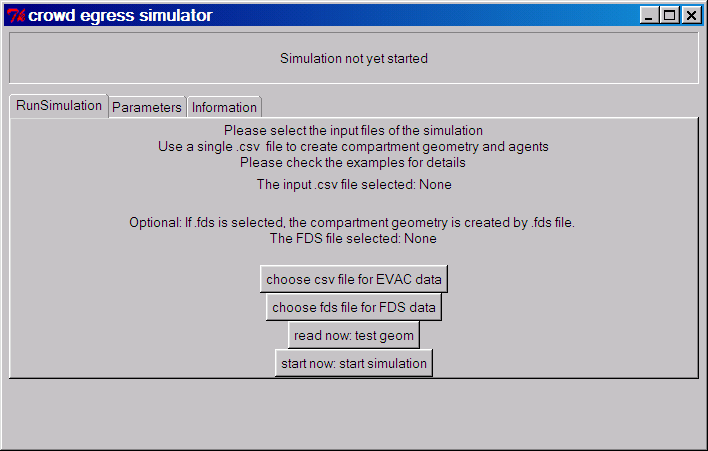
\includegraphics[clip,scale=0.3]{img/gui.PNG}} \caption{In Tkinter Screen}

\label{Fig_TkScreen} 
\end{figure}

\noindent \textbf{In Pygame Screen}: When pygame screen is displayed,
press keys to adjust the display features and visualize entity data.
There are two sections in pygame screen. One section is called TestGeom,
where users can visualize compartment geometric settings and modify
them manually. Users can also dump geometric data (e.g., wall data
and door data) into csv file by selecting the item <OutputData> in
the menu bar. The data can also be briefly shown in the screen by
selecting the item <ShowData> in the menu bar. If users click <Simulation>,
then the simulation starts and the program goes to the second section
called RunSimulation. 

\begin{figure}
\centerline{\includegraphics[clip,scale=0.3]{img/massEgress}} \caption{An Example in Pygame: TestGeom Window}

\label{Fig_Example_TestGeom} 
\end{figure}

The other section is RunSimulation, in which the evac simulation is
started and visualized on the screen. User can pause the simulation,
but cannot rewind it in current version (Version 2.0). A binary data
file is created when the simulation runs and users can also visualize
the data by using our visualizer component. 

In both phase of TestGeom and RunSimulation, there are hot keys defined.
Use pageup/pagedown to zoom in or zoom out the entities in screen.
Use space key to pause the simulation. Use arrows to move the entities
vertically or horizonally in screen. Use 1/2/3 in number panel (Right
side in the keyboard) to display the door or exit data on the screen.

\textbf{Try Examples}: There are currently several examples in the repo.
Please execute run.bat in the subfolders to run the example. The examples
are run by using non-gui method. Users can also learn how to write
the .csv files from the examples.

\begin{figure}
\centerline{\includegraphics[clip,scale=0.3]{img/massEgress2}}
\caption{An Example in Pygame: Simulation Window}

\label{Fig_Example_Sim} 
\end{figure}

%\chapter*{Acknowledgements}
%\addcontentsline{toc}{chapter}{Acknowledgements}

%\noindent The authors are thankful to Dr.\ Peter Luh and Dr.\ Kerry Marsh for helpful comments on earlier work in University of Connecticut.   The authors are also grateful to Dr.\ Timo Korhonen for helpful discussion in simulation work of FDS+Evac.  The author appreciates the  research program funded by NSF Grant CMMI-1000495 (NSF Program Name: Building Emergency Evacuation - Innovative Modeling and Optimization).

\clearpage{}

\newpage{}

\addcontentsline{toc}{chapter}{References} %\renewcommand{\bibname}{References}

\begin{thebibliography}{References}

%\bibitem{Adam17}J. Ba�gate, J. Dugdale, C. Adam, E. Beck, \textquotedblleft A Review on the Influence of Social Attachment on Human Mobility During Crises,\textquotedblright{} T2-Analytical Modelling and Simulation Proceedings of the 14th ISCRAM Conference, Albi, France, May 2017.

%\bibitem{SMV_UserGuide} Forney, G.P., ``Smokeview, A Tool for Visualizing Fire Dynamics Simulation Data, Volume I: User's Guide'', NIST Special Publication 1017-1 6th Edition, National Institute of Standards and Technology, Gaithersburg, MA, June 2016, 188~p. 

%\bibitem{SMV_TechGuide} Forney, G.P., ``Smokeview (Version 6.1.5) - A Tool for Visualizing Fire Dynamics Simulation Data, Volume II: Technical Reference Guide'', NIST Special Publication 1017-1, National Institute of Standards and Technology, Gaithersburg, MA, August 2013, 70~p. 

\bibitem{SMV_VVGuide} Forney, G.P., ``Smokeview (Version 6.1.5)
- A Tool for Visualizing Fire Dynamics Simulation Data, Volume III:
Verification Guide'', NIST Special Publication 1017-3, National Institute
of Standards and Technology, Gaithersburg, MA, November 2013, 88~p.

\bibitem{Helbing02} Helbing, D., Farkas, I., Moln�r, P., and Vicsek,T.,
``Simulating of Pedestrian Crowds in Normal and Evacuation Situations'',
\emph{Pedestrian and Evacuation Dynamics}, Schreckenberg, M. and Sharma,
S.D. (eds.), Springer, Berlin, 2002, pp.~21--58.

\bibitem{Helbing00} Helbing, D., Farkas, I., and Vicsek, T., ``Simulating
dynamical features of escape panic'', \emph{Nature} 407: 487--490
(2000). % Next is for book

\bibitem{Helbing95} Helbing, D., and Moln�r, P., ``Social force
model for pedestrian dynamics'', \emph{Physical Review E} 51: 4282--4286
(1995). 

\bibitem{IMO07} IMO, ``Guidelines for Evacuation Analyses for New
and Existing Passenger Ships'', MSC/Circ.1238, International Maritime
Organization, London, UK, 30 October 2007.

\bibitem{Korhonen09} Korhonen, T. and Hostikka, S., ``Fire Dynamics
Simulator with Evacuation: FDS+Evac Technical Reference and User's
Guide'', VTT Working Papers 119, VTT Technical Research Centre of
Finland, Espoo, Finland, 2011.

\bibitem{Lakoba05}T. I. Lakoba, D. J. Kaup, N. M. Finkelstein, \textquotedblleft Modifications
of the Helbing-Moln�r-Farkas-Vicsek Social Force Model for Pedestrian
Evolution,\textquotedblright{} Simulation, Vol. 81, Issue 5, pp. 339-352,
May 2005.

\bibitem{FDS_UserGuide} McGrattan, K., Hostikka, S., McDermott, R.,
Floyd, J., Weinschenk, C., and Overholt, K., ``Fire Dynamics Simulator,
User's Guide'', NIST Special Publication 1019 6th Ed., National Institute
of Standards and Technology, Gaithersburg, MA, October 2016, 290~p. 

\bibitem{Proulx1993} Proulx, G., ``A Stress Model for People Facing
a Fire'', \emph{Journal of Environmental Psychology} 13: 137--147,
1993.

%\bibitem{Simulex96} ``Simulex: Evacuation Modelling Software, User's Guide'', Integrated Environmental Solutions Ltd., Glasgow, Scotland,
UK, 1996, 48~p. 

\bibitem{Wang16} P.Wang, ''Understanding Social Force Model in Psychological 
Principles of Collective Behavior,'' arXiv:1605.05146, Master Thesis, 2016.  

\bibitem{Wang20} P. Wang and X. Wang, ''Social Force in Pedestrian Crowd,'' arXiv:2109.12597, 2021.  

\end{thebibliography}

\end{document}
